\documentclass[12pt,twoside]{article}
\usepackage[dvipsnames]{xcolor}
\usepackage{tikz,graphicx,amsmath,amsfonts,amscd,amssymb,bm,cite,epsfig,epsf,url}
\usepackage[hang,flushmargin]{footmisc}
\usepackage[colorlinks=true,urlcolor=blue,citecolor=blue]{hyperref}
\usepackage{amsthm,multirow,wasysym,appendix}
\usepackage{array,subcaption} 
% \usepackage[small,bf]{caption}
\usepackage{bbm}
\usepackage{pgfplots}
\usetikzlibrary{spy}
\usepgfplotslibrary{external}
\usepgfplotslibrary{fillbetween}
\usetikzlibrary{arrows,automata}
\usepackage{thmtools}
\usepackage{blkarray} 
\usepackage{textcomp}
\usepackage[left=0.8in,right=1.0in,top=1.0in,bottom=1.0in]{geometry}

\usepackage{times}
\usepackage{amsfonts}
\usepackage{amsmath}
\usepackage{latexsym}
\usepackage{color}
\usepackage{graphics}
\usepackage{enumerate}
\usepackage{amstext}
\usepackage{blkarray}
\usepackage{url}
\usepackage{epsfig}
\usepackage{bm}
\usepackage{hyperref}
\hypersetup{
    colorlinks=true,
    linkcolor=blue,
    filecolor=magenta,      
    urlcolor=blue,
}
\usepackage{textcomp}
\usepackage[left=0.8in,right=1.0in,top=1.0in,bottom=1.0in]{geometry}
\usepackage{mathtools}
\usepackage{minted}

%% Probability operators and functions
%
% \def \P{\mathrm{P}}
\def \P{\mathrm{P}}
\def \E{\mathrm{E}}
\def \Var{\mathrm{Var}}
\let\var\Var
\def \Cov {\mathrm{Cov}} \let\cov\Cov
\def \MSE {\mathrm{MSE}} \let\mse\MSE
\def \sgn {\mathrm{sgn}}
\def \R {\mathbb{R}}
\def \C {\mathbb{C}}
\def \N {\mathbb{N}}
\def \Z {\mathbb{Z}}
\def \cV {\mathcal{V}}
\def \cS {\mathcal{S}}
\DeclareMathOperator*{\argmin}{arg\,min}
\DeclareMathOperator*{\argmax}{arg\,max}
\newcommand{\red}[1]{\textcolor{red}{#1}}
\newcommand{\blue}[1]{\textcolor{blue}{#1}}
\newcommand{\green}[1]{\textcolor{ForestGreen}{ #1}}
\newcommand{\fuchsia}[1]{\textcolor{RoyalPurple}{ #1}}

%
%% Probability distributions
%
%\def \Bern    {\mathrm{Bern}}
%\def \Binom   {\mathrm{Binom}}
%\def \Exp     {\mathrm{Exp}}
%\def \Geom    {\mathrm{Geom}}
%\def \Norm    {\mathcal{N}}
%\def \Poisson {\mathrm{Poisson}}
%\def \Unif    {\mathrm {U}}
%
\newcommand{\bdb}[1]{\textcolor{red}{#1}}

\newcommand{\ml}[1]{\mathcal{ #1 } }
\newcommand{\wh}[1]{\widehat{ #1 } }
\newcommand{\wt}[1]{\widetilde{ #1 } }
\newcommand{\conj}[1]{\overline{ #1 } }
\newcommand{\rnd}[1]{\tilde{ #1 } }
\newcommand{\rv}[1]{ \rnd{ #1}  }
\newcommand{\rx}{\rnd{ x}  }
\newcommand{\ry}{\rnd{ y}  }
\newcommand{\ra}{\rnd{ a}  }
\newcommand{\rb}{\rnd{ b}  }
\newcommand{\rpc}{\widetilde{ pc}  }

\def \cnd {\, | \,}
\def \Id { I }
\def \J {\mathbf{1}\mathbf{1}^T}

\newcommand{\op}[1]{\operatorname{#1}}
\newcommand{\setdef}[2]{ := \keys{ #1 \; | \; #2 } }
\newcommand{\set}[2]{ \keys{ #1 \; | \; #2 } }
\newcommand{\sign}[1]{\op{sign}\left( #1 \right) }
\newcommand{\trace}[1]{\op{tr}\left( #1 \right) }
\newcommand{\tr}[1]{\op{tr}\left( #1 \right) }
\newcommand{\inv}[1]{\left( #1 \right)^{-1} }
\newcommand{\abs}[1]{\left| #1 \right|}
\newcommand{\sabs}[1]{| #1 |}
\newcommand{\keys}[1]{\left\{ #1 \right\}}
\newcommand{\sqbr}[1]{\left[ #1 \right]}
\newcommand{\sbrac}[1]{ ( #1 ) }
\newcommand{\brac}[1]{\left( #1 \right) }
\newcommand{\bbrac}[1]{\big( #1 \big) }
\newcommand{\Bbrac}[1]{\Big( #1 \Big)}
\newcommand{\BBbrac}[1]{\BIG( #1 \Big)}
\newcommand{\MAT}[1]{\begin{bmatrix} #1 \end{bmatrix}}
\newcommand{\sMAT}[1]{\left(\begin{smallmatrix} #1 \end{smallmatrix}\right)}
\newcommand{\sMATn}[1]{\begin{smallmatrix} #1 \end{smallmatrix}}
\newcommand{\PROD}[2]{\left \langle #1, #2\right \rangle}
\newcommand{\PRODs}[2]{\langle #1, #2 \rangle}
\newcommand{\der}[2]{\frac{\text{d}#2}{\text{d}#1}}
\newcommand{\pder}[2]{\frac{\partial#2}{\partial#1}}
\newcommand{\derTwo}[2]{\frac{\text{d}^2#2}{\text{d}#1^2}}
\newcommand{\ceil}[1]{\lceil #1 \rceil}
\newcommand{\Imag}[1]{\op{Im}\brac{ #1 }}
\newcommand{\Real}[1]{\op{Re}\brac{ #1 }}
\newcommand{\norm}[1]{\left|\left| #1 \right|\right| }
\newcommand{\norms}[1]{ \| #1 \|  }
\newcommand{\normProd}[1]{\left|\left| #1 \right|\right| _{\PROD{\cdot}{\cdot}} }
\newcommand{\normTwo}[1]{\left|\left| #1 \right|\right| _{2} }
\newcommand{\normTwos}[1]{ \| #1  \| _{2} }
\newcommand{\normZero}[1]{\left|\left| #1 \right|\right| _{0} }
\newcommand{\normTV}[1]{\left|\left| #1 \right|\right|  _{ \op{TV}  } }% _{\op{c} \ell_1} }
\newcommand{\normOne}[1]{\left|\left| #1 \right|\right| _{1} }
\newcommand{\normOnes}[1]{\| #1 \| _{1} }
\newcommand{\normOneTwo}[1]{\left|\left| #1 \right|\right| _{1,2} }
\newcommand{\normF}[1]{\left|\left| #1 \right|\right| _{\op{F}} }
\newcommand{\normLTwo}[1]{\left|\left| #1 \right|\right| _{\ml{L}_2} }
\newcommand{\normNuc}[1]{\left|\left| #1 \right|\right| _{\ast} }
\newcommand{\normOp}[1]{\left|\left| #1 \right|\right|  }
\newcommand{\normInf}[1]{\left|\left| #1 \right|\right| _{\infty}  }
\newcommand{\proj}[1]{\mathcal{P}_{#1} \, }
\newcommand{\diff}[1]{ \, \text{d}#1 }
\newcommand{\vc}[1]{\boldsymbol{\vec{#1}}}
\newcommand{\rc}[1]{\boldsymbol{#1}}
\newcommand{\vx}{\vec{x}}
\newcommand{\vy}{\vec{y}}
\newcommand{\vz}{\vec{z}}
\newcommand{\vu}{\vec{u}}
\newcommand{\vv}{\vec{v}}
\newcommand{\vb}{\vec{\beta}}
\newcommand{\va}{\vec{\alpha}}
\newcommand{\vaa}{\vec{a}}
\newcommand{\vbb}{\vec{b}}
\newcommand{\vg}{\vec{g}}
\newcommand{\vw}{\vec{w}}
\newcommand{\vh}{\vec{h}}
\newcommand{\vnu}{\vec{\nu}}
\newcommand{\rvnu}{\vc{\nu}}

\newtheorem{theorem}{Theorem}[section]
% \declaretheorem[style=plain,qed=$\square$]{theorem}
\newtheorem{corollary}[theorem]{Corollary}
\newtheorem{definition}[theorem]{Definition}
\newtheorem{lemma}[theorem]{Lemma}
\newtheorem{remark}[theorem]{Remark}
\newtheorem{algorithm}[theorem]{Algorithm}

% \theoremstyle{definition}
%\newtheorem{example}[proof]{Example}
%\declaretheorem[style=definition,qed=$\triangle$,sibling=definition]{example}
%\declaretheorem[style=definition,qed=$\bigcirc$,sibling=definition]{application}

%
%% Typographic tweaks and miscellaneous
%\newcommand{\sfrac}[2]{\mbox{\small$\displaystyle\frac{#1}{#2}$}}
%\newcommand{\suchthat}{\kern0.1em{:}\kern0.3em}
%\newcommand{\qqquad}{\kern3em}
%\newcommand{\cond}{\,|\,}
%\def\Matlab{\textsc{Matlab}}
%\newcommand{\displayskip}[1]{\abovedisplayskip #1\belowdisplayskip #1}
%\newcommand{\term}[1]{\emph{#1}}
%\renewcommand{\implies}{\;\Rightarrow\;}

% My macros

\def\Kset{\mathbb{K}}
\def\Nset{\mathbb{N}}
\def\Qset{\mathbb{Q}}
\def\Rset{\mathbb{R}}
\def\Sset{\mathbb{S}}
\def\Zset{\mathbb{Z}}
\def\squareforqed{\hbox{\rlap{$\sqcap$}$\sqcup$}}
\def\qed{\ifmmode\squareforqed\else{\unskip\nobreak\hfil
\penalty50\hskip1em\null\nobreak\hfil\squareforqed
\parfillskip=0pt\finalhyphendemerits=0\endgraf}\fi}

%\DeclareMathOperator*{\E}{\rm E}
%\DeclareMathOperator*{\argmax}{\rm argmax}
%\DeclareMathOperator*{\argmin}{\rm argmin}
%\DeclareMathOperator{\sgn}{sign}
\DeclareMathOperator{\supp}{supp}
\DeclareMathOperator{\last}{last}
%\DeclareMathOperator{\sign}{\sgn}
\DeclareMathOperator{\diag}{diag}
\providecommand{\abs}[1]{\lvert#1\rvert}
\providecommand{\norm}[1]{\lVert#1\rVert}
\def\vcdim{\textnormal{VCdim}}
\DeclareMathOperator*{\B}{\textbf{B}}

%\DeclarePairedDelimiter\ceil{\lceil}{\rceil}
%\DeclarePairedDelimiter\floor{\lfloor}{\rfloor}

\newcommand{\cX}{{\mathcal X}}
\newcommand{\cY}{{\mathcal Y}}
\newcommand{\cA}{{\mathcal A}}
\newcommand{\ignore}[1]{}
\newcommand{\bi}{\begin{itemize}}
\newcommand{\ei}{\end{itemize}}
\newcommand{\be}{\begin{enumerate}}
\newcommand{\ee}{\end{enumerate}}
\newcommand{\bd}{\begin{description}}
\newcommand{\ed}{\end{description}}
\newcommand{\h}{\widehat}
\newcommand{\e}{\epsilon}
\newcommand{\mat}[1]{{\mathbf #1}}
%\newcommand{\R}{\mat{R}}
\newcommand{\0}{\mat{0}}
\newcommand{\M}{\mat{M}}

\newcommand{\D}{\mat{D}}
\renewcommand{\r}{\mat{r}}
\newcommand{\x}{\mat{x}}
\renewcommand{\u}{\mat{u}}
\renewcommand{\v}{\mat{v}}
\newcommand{\w}{\mat{w}}
\renewcommand{\H}{\text{0}}
\newcommand{\T}{\text{1}}
%\newcommand{\set}[1]{\{#1\}}
\newcommand{\xxi}{{\boldsymbol \xi}}
\newcommand{\ssigma}{{\boldsymbol \sigma}}
\newcommand{\Alpha}{{\boldsymbol \alpha}}
\newcommand{\tts}{\tt \small}
\newcommand{\hint}{\emph{hint}}
\newcommand{\matr}[1]{\bm{#1}}     % ISO complying version
\newcommand{\vect}[1]{\bm{#1}} % vectors

%\newcommand{\Var}{\mathrm{Var}}
%\newcommand{\Cov}{\mathrm{Cov}}

% New commands
\newcommand{\SP}{\mathbf{S}_{+}^n}
\newcommand{\Proj}{\mathcal{P}_{\mathcal{S}}}
\DeclarePairedDelimiterX{\inp}[2]{\langle}{\rangle}{#1, #2}
\newtheorem{proof}{Proof}


\begin{document}

\begin{center}
{\large{\textbf{Homework 6}} } \vspace{0.2cm}\\
Due April 5 at 11 pm
\end{center}
Yves Greatti - yg390\\

\begin{enumerate}

\item (Gradient descent and ridge regression) In this problem we study the iterations of gradient descent applied to the ridge-regression cost function
\begin{align}
\min_{\beta \in \R^p} \frac{1}{2}\normTwo{y-X^T\beta}^2 + \frac{\lambda}{2}\normTwo{\beta}^2,
\end{align}
where $X \in \R^{p \times n}$ is a fixed feature matrix and $y\in \R^{n}$ is a response vector. (The factor of 1/2 is just there to make calculations a bit cleaner.)
\begin{enumerate}
\item Derive a closed form expression for the value of the estimated coefficient $\beta^{\brac{k}}$ at the $k$th iteration of gradient descent initialized at the origin in terms of the SVD of $X$ when the step size is constant. \\

The gradient-descent updates are:
\begin{align*}
		\beta^{(k+1)}	&=	\beta^{(k)} - \; \alpha_k \nabla_{\beta} f(\beta^{(k)})	\\
					&=	\beta^{(k)}  - \alpha_k (X X^T \beta^{(k)} - X y +  \lambda \beta^{(k)}) \\
					&=    ((1- \lambda \alpha_k) I  - \alpha_k X X^T) \beta^{(k)}  +  \alpha_k  X y  \\
					&=	\big( ( 1 - \alpha \lambda) I - \alpha X X^T  \big)^{k+1} \beta^{(0)}  +	\alpha \sum_{i=0}^k \big( (1 - \alpha \lambda) I - \alpha X X^T \big)^i X y \\
					&=	\alpha \sum_{i=0}^k \big( (1 - \alpha \lambda) I - \alpha X X^T \big)^i X y \
\end{align*}
since the step size $\alpha_k = \alpha$ is constant and $\beta^{(0)}$ is the zero vector (initialization at the origin).    
Let the svd of $X = U S V^T$ then 
\begin{align*}
		\beta^{(k+1)}	&= \alpha  \sum_{i=0}^k \big( (1 - \alpha \lambda) I - \alpha U S^2 U^T  \big)^i U S V^T y \\
\end{align*}

Assuming $p \le n$ and $X$ is full rank, $UU^T = U^T U = I$ and we have:
\begin{align*}
	\beta^{(k+1)}	&=  \alpha  \sum_{i=0}^k \big( (1  - \alpha \lambda) UU^T- \alpha U S^2 U^T \big)^i U S V^T y \\
				&= \alpha U   \sum_{i=0}^k \big( ( 1 - \alpha \lambda) I - \alpha S^2  \big)^i  S V^T y \\
				&=  \alpha U   \text{diag}_{j=1}^p \sum_{i=0}^k \big(  1 - \alpha (s_j^2 + \lambda)  \big)^i  S V^T y \\
				&=  U   \text{diag}_{j=1}^p \frac{ 1 - ( 1 - \alpha (s_j^2 + \lambda))^{k+1} s_j}{s_j^2 + \lambda}  \;  V^T y \\ 
\end{align*}

\item Under what condition on the step size does gradient descent converge to the ridge-regression coefficient estimate as $k \rightarrow \infty$?\\
If step size $\alpha$ is small enough: $0 < \alpha < \frac{2} {\lambda + s_1^2} \le \frac{2} {\lambda + s_j^2} \rightarrow |1 - \alpha (s_j^2 + \lambda)| < 1$ then
 $\lim_{k \rightarrow \infty} (1 - \alpha (s_j^2 + \lambda))^k =0, j=1, \dots ,p $, gradient descent converges to:
\begin{align*}
	\lim_{k \rightarrow \infty} \beta^{(k)}	&= U  \;  \text{diag}_{j=1}^p \bigg( \frac{s_j} {s_j^2 + \lambda} \bigg)  V^T y \\
									&= U (S^2 + \lambda I)^{-1} S^2 V^T y
\end{align*}
which are the ridge-regression coefficient estimates.

\item Assume the following additive model for the data:  
\begin{align}
\ry_{\op{train}} := X^T \beta_{\op{true}} + \rnd{z}_{\op{train}},
\end{align}
where $\rnd{z}_{\op{train}}$ is modeled as an $n$-dimensional iid Gaussian vector with zero mean and variance $\sigma^2$. What is the distribution of the estimated coefficient $\rnd{\beta}^{\brac{k}}$ at the $k$th iteration of gradient descent initialized at the origin?\\
Using the expression of the estimated coefficients from part a, we now have:

\begin{align*}
	\rnd{\beta}^{\brac{k}} &=  U  \text{diag}_{j=1}^p \frac{ 1 - ( 1 - \alpha (s_j^2 + \lambda))^{k} s_j}{s_j^2 + \lambda}  \;  V^T (X^T \beta_{\op{true}} + \rnd{z}_{\op{train}} )\\
					&=  U  \text{diag}_{j=1}^p \frac{ 1 - ( 1 - \alpha (s_j^2 + \lambda))^{k} s_j}{s_j^2 + \lambda}  \;  V^T (V S U^T \beta_{\op{true}} + \rnd{z}_{\op{train}} )\\
					&=  U  \text{diag}_{j=1}^p \frac{ 1 - ( 1 - \alpha (s_j^2 + \lambda))^{k} s_j^2}{s_j^2 + \lambda}  \; U^T \beta_{\op{true}} 
					+      U  \text{diag}_{j=1}^p \frac{ 1 - ( 1 - \alpha (s_j^2 + \lambda))^{k} s_j}{s_j^2 + \lambda}  \;  V^T  \rnd{z}_{\op{train}} \\
\end{align*}
Using theorem 8,6 from the notes on PCA, then  the estimated coefficient $\rnd{\beta}^{\brac{k}}$ at the $k$th iteration of gradient descent initialized at the origin have is a Gaussian random vector  with mean:

$$ \beta_{\text{GD}}  = \sum_{j=1}^p  \frac{ 1 - ( 1 - \alpha (s_j^2 + \lambda))^{k} s_j^2}{s_j^2 + \lambda}  \PROD{u_j}{\beta_{\op{true}}} u_j $$
and covariance matrix

$$ \Sigma_{\text{GD}} = \sigma^2 U  \text{diag}_{j=1}^p \frac{ (1 - ( 1 - \alpha (s_j^2 + \lambda))^{k})^2 s_j^2}{(s_j^2 + \lambda)^2}  U^T $$

\item Complete the script \emph{RR\_GD\_landscape.py} in order to verify your answer to the previous question. Report the figures generated by the script.
\end{enumerate}
 
\newpage

\item  (Climate modeling) In this problem we model temperature trends using a linear regression model. The file 
\texttt{t\_data.csv} contains the maximum temperature measured
  each month in Oxford from 1853-2014.  We will use the first
  150 years of data (the first $150\cdot 12$ data points) as a training set, and
  the remaining 12 years as a test set.

 In order to fit the evolution of the temperature over the years, we fit the following model
  \begin{align}
  y[t] = a + bt + c \cos(2\pi t/T) + d\sin(2\pi  t/T)
  \end{align}
  where $a,b,c,d\in\R$, $y[t]$ denotes the maximum temperature in Celsius during month $t$ of the dataset (with $t$ starting from $0$ and ending at $162\cdot 12-1$).
   
  \begin{enumerate}
  \item What is the number of parameters in your model and how many data points do you have to fit the model? Are you worried about overfitting?\\
  The number of parameters if $4$ much less than the number of training samples $150\cdot 12 = 1800$, so we have enough samples compared to the number of parameters and our linear regression model will not overfit as there are enough data points.
  Since we want to model the trend of the temperature over the years we have enough datapoints to detect the trend of the  temperature. If we did not have enough points compared to the number of parameters our model will overfit, fitting mostly the noise.
  
  \item Fit the model using least squares on the training set to
    find the coefficients for values of $T$ equal to 1,2,\ldots,20. Which of these models provides a better fit? Explain why this is the case. In the remaining question we will fix $T$ to the value $T^{\ast}$ that provides a better fit.\\ \\

    When we plot the training errors we find out the model with the better fit is T=12. This is the value of T for which estimate coefficients  corresponding to the cosine and sine  terms
    are the maximum in amplitude, allowing to better fit the oscillations of the temperatures over the years. $T=12$ corresponds also to the number of months in a year and could be seen as the period to which the temperatures fall in  
    the same range from one year to the other for the corresponding month.
    
  \item Produce two plots comparing the actual maximum temperatures with
    the ones predicted by your model for $T:=T^{\ast}$; one for the training set and one for the test set. \\
    
	\begin{figure}[H]
		\centering
		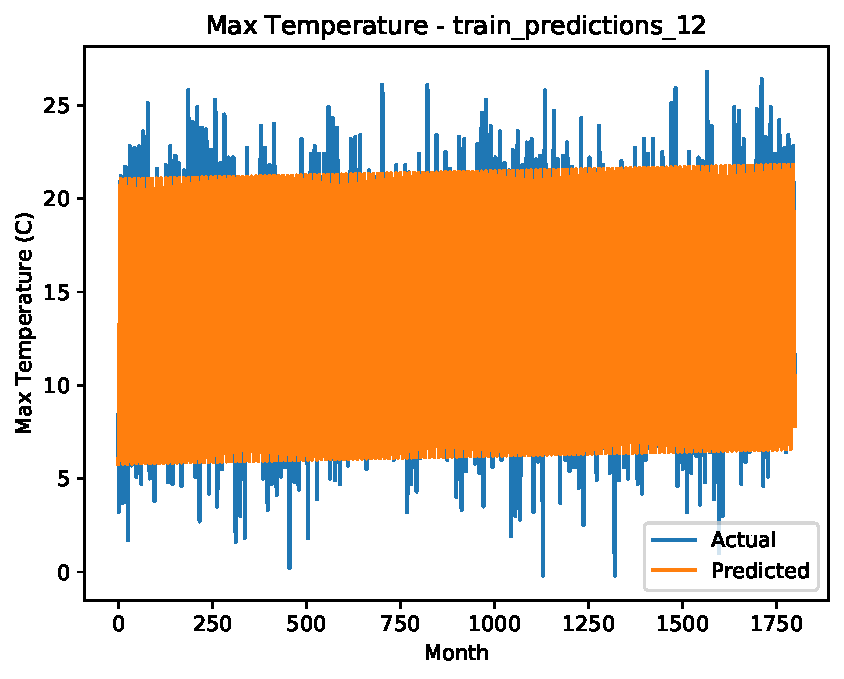
\includegraphics[width=200pt]{code/Q2/train_predictions_12_fit.pdf}
		\caption{Actual and predicted max. temperatures from 1853-2014 \newline for $T=12$ on the training set.}
	\end{figure}

	\begin{figure}[H]
		\centering
		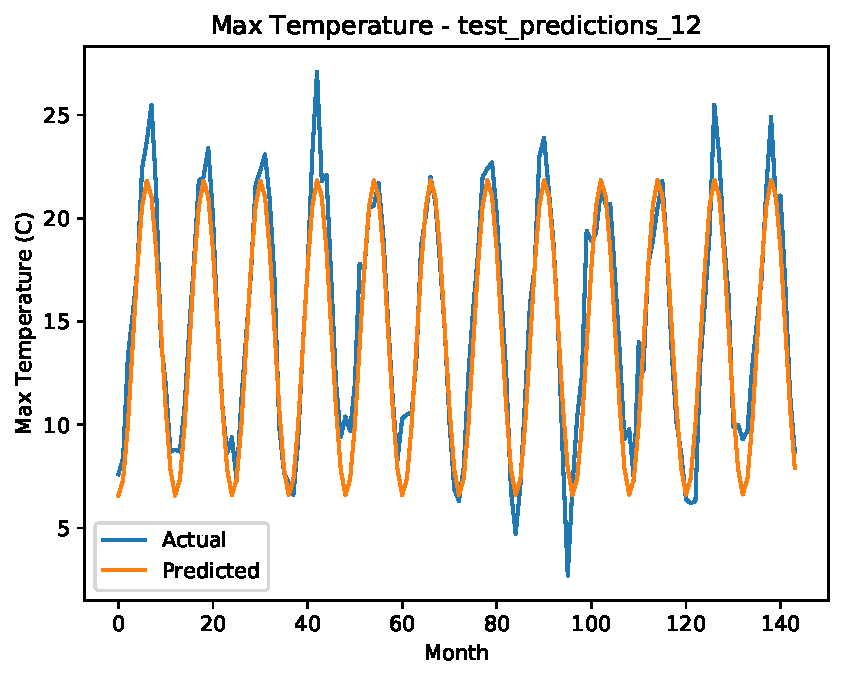
\includegraphics[width=200pt]{code/Q2/test_predictions_12_fit.pdf}
		\caption{Actual and predicted max. temperatures from 1853-2014 \newline for $T=12$ on the test set.}
	\end{figure}
    
 \item Fit the modified model  
   \begin{align}
  y[t] = a + bt + d \sin(2\pi t/T^{\ast})
  \end{align}
and plot the fit to the training data as in the previous question. Explain why it is better to also include a cosine term in the model.\\ \\

Not having the cosine term simplify the model but we are no longer capturing all the frequencies of the fundamental seasonal frequency of the temperatures. So it is better to combine sine and cosine terms to span more frequencies. 

	\begin{figure}[H]
		\centering
		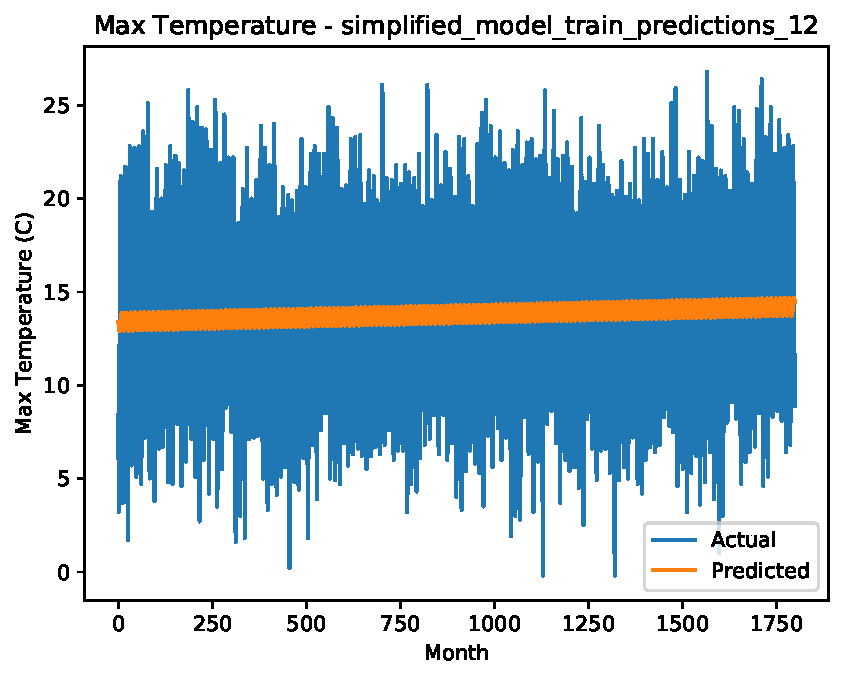
\includegraphics[width=200pt]{code/Q2/simplified_model_train_predictions_12_fit.pdf}
		\caption{Actual and predicted max. temperatures from 1853-2014 \newline for $T=12$ on the training set using the model $y[t] = a + bt + d \sin(2\pi t/T^{\ast})$.}
	\end{figure}

	\begin{figure}[H]
		\centering
		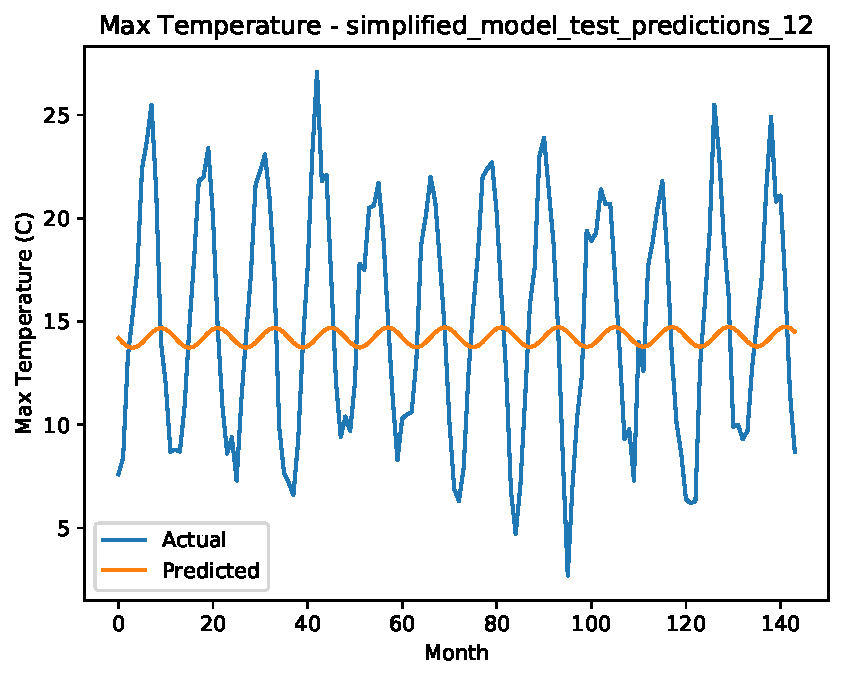
\includegraphics[width=200pt]{code/Q2/simplified_model_test_predictions_12_fit.pdf}
		\caption{Actual and predicted max. temperatures from 1853-2014 \newline for $T=12$ on the test set $y[t] = a + bt + d \sin(2\pi t/T^{\ast})$.}
	\end{figure}


   \item Provide an intuitive interpretation of the coefficients $a$, $b$, $c$ and $d$, and the corresponding features. According to your model, are temperatures rising in Oxford? By how much?\\
   \begin{itemize}
   	\item a is the intercept or expected mean of the temperatures over the years
	\item b corresponds to the trend or drift of the temperatures
	\item c and d are related to the seasonal frequencies of the temperatures, they are included to capture the vertical or horizontal shift of these temperatures over time and their periodicity
   \end{itemize}
   If we look at the trend of the predicted temperatures on the training set (see fig. 3) or if we use a value of $T$ which corresponds to a model less sensitive to the seasonality of the temperatures, we observe that the temperatures
   are increasing in Oxford by 2-3 degrees.
   
  \end{enumerate}
   
 \item (Sines and cosines)
  Let $x:[-1/2,1/2)\to\R $ be a real-valued square-integrable function defined on the interval $[-1/2,1/2)$, i.e. $x\in L_2[-1/2,1/2)$. The Fourier series coefficients of $x$, are given by
\begin{align}
\hat{x}[k] & :=  \PROD{x}{\phi_k} = \int_{-1/2}^{1/2} x(t) \exp \brac{- i2 \pi k t}  \diff{t}, \quad k \in \Z,
\end{align}
and the corresponding Fourier series of order $k_c$ equals
\begin{align}
\ml{F}_{k_c}\{x\}(t) = \sum_{k=-k_c}^{k_c} \hat{x}[k] \exp \brac{i 2 \pi k t}.
\end{align}
As we will discuss in class, this is a representation of $x$ in a basis of complex exponentials. In this problem we show that for real signals the Fourier series is equivalent to a representation in terms of cosine and sine functions.
  \begin{enumerate}
  \item Prove that $\hat{x}[k]=\overline{\hat{x}[-k]}$
    for all $k\in\Z$. [Hint: What is $\overline{e^{it}}$?]\\
    \begin{align*}
    	\overline{\hat{x}[-k]} 	&= 	\overline{  \int_{-1/2}^{1/2} x(t) \exp \brac{ i 2 \pi k t}  \diff{t} } \\
					&=	 \int_{-1/2}^{1/2} \overline{x(t)} \overline{ \exp \brac{ i2 \pi k t} } \diff{t} \\
					&=	 \int_{-1/2}^{1/2} x(t)  \exp \brac{ -i 2 \pi k t} \diff{t} \\
					&= 	 \hat{x}[k] \\
    \end{align*}
    
    
  \item Show that the Fourier series of $x$ of order $k_c$ can be written as
    $$\ml{F}_{k_c}\{x\}(t) = a_0 + \sum_{k=1}^{k_c} a_k\cos(2\pi
    kt)+b_k\sin(2\pi kt),$$
    for some $a_0,\ldots,a_k,b_1,\ldots,b_k\in\R$. [Hint: Group terms
      in $\ml{F}_{k_c}\{x\}(t)$ corresponding to $\pm k$ and use previous
      part.  What is the real part of $zw$ for $z,w\in\C $?]
      
    \begin{align*}
		\ml{F}_{k_c}\{x\}(t) 	&=	\sum_{k=-k_c}^{k_c} \hat{x}[k] \exp \brac{i 2 \pi k t} \\
						&= 	\hat{x}[0] +  \sum_{k=-k_c}^{-1} \hat{x}[k] \exp \brac{i 2 \pi k t} + \sum_{k=1}^{k_c} \hat{x}[k] \exp \brac{i 2 \pi k t} \\
						&= 	\hat{x}[0] +  \sum_{k=k_c}^{1} \hat{x}[-k] \exp \brac{- i 2 \pi k t} + \sum_{k=1}^{k_c} \hat{x}[k] \exp \brac{i 2 \pi k t} \\
						&=	\hat{x}[0] +   \sum_{k=1}^{k_c} (\hat{x}[-k] \exp \brac{- i 2 \pi k t} +  \hat{x}[k] \exp \brac{i 2 \pi k t} ) \\
						&=	\hat{x}[0] +   \sum_{k=1}^{k_c} (\overline{ \hat{x}[k] } \exp \brac{- i 2 \pi k t} +  \hat{x}[k] \exp \brac{i 2 \pi k t} ) \text{ ~ using part a } \\
   \end{align*}
Given two complex numbers $z = a + i b$ and $w = c + id$, we have $zw = ac - bd + i (ad + bc)$ and $\overline{z} \; \overline{w} = ac - bd - i (ad + bc)$ giving that $z w + \overline{z} \overline{w} = 2 (ac - bd)$.
Let  $z_k = \hat{x}[k]$ and $w_k =     \exp \brac{i 2 \pi k t} $ thus
   \begin{align*}
   	\ml{F}_{k_c}\{x\}(t) 		&=  \hat{x}[0] +  \sum_{k=1}^{k_c} 2 (\Real{ \hat{x}[k]} \cos{ 2 \pi k t} - \Imag{\hat{x}[k] }  \sin{ 2 \pi k t} ) \\
						&= \hat{x}[0] +  \sum_{k=1}^{k_c} (2 \Real{ \hat{x}[k]}) \cos{ 2 \pi k t} + (-2  \Imag{\hat{x}[k] } ) \sin{ 2 \pi k t}  \\
						&= \hat{x}[0] +   \sum_{k=1}^{k_c} a_k \cos(2\pi k t) + b_k \sin(2\pi k t) \\
   \end{align*}
   
  \item Give
    expressions for the coefficients $a_k,b_k$ for $k\geq 1$ from the
    previous part as real integrals. Interpret them in terms of inner products.
    
    From the definition 
   \begin{align*}
  				 \hat{x}[k] 	&= \PROD{x}{\phi_k} = \int_{-1/2}^{1/2} x(t) \exp \brac{- i2 \pi k t}  \diff{t}   \text{ for } k\geq 1\\
				 		&=  	\int_{-1/2}^{1/2} x(t) (\cos(2\pi k t) + i \sin(2\pi k t)) \diff{t} \\
						&=	 \int_{-1/2}^{1/2} x(t)  \cos(2\pi k t) \diff{t} + i \int_{-1/2}^{1/2} x(t) \sin(2\pi k t) \diff{t} \\
						&=	\Real{ \hat{x}[k]} + i   \Imag{\hat{x}[k] } \\			
   \end{align*}
   thus 
   $$a_k =2 \int_{-1/2}^{1/2} x(t)  \cos(2\pi k t) \diff{t} = 2  \PROD{x}{ \cos(2\pi k t) } =  2  \PROD{x}{\Real{ \phi_k}} $$ 
   and $$b_k =  2 \int_{-1/2}^{1/2} x(t)   \sin(2\pi k t) \diff{t} = 2  \PROD{x}{ \sin(2\pi k t) } =  2  \PROD{x}{\Imag{ \phi_k}}$$.
          
  \item Suppose $x(t)=\cos(2\pi(t+\phi))$ for some fixed
    $\phi\in\R$.  What are the Fourier coefficients of $x$?
  \item Suppose that $f$ is also even (i.e., $x(-t)=x(t)$).  Prove
    that the Fourier coefficients are all real (i.e., that
    $\hat{x}[k]\in\R$ for all $k\in\Z$).
    
    Using part a
      \begin{align*}
      	\overline{\hat{x}[k]}	&= 	\hat{x}[-k] \\
					&= 	\int_{-1/2}^{1/2} x(t) \exp \brac{i 2 \pi k t}  \diff{t} \\
					&= 	\int_{1/2}^{-1/2} x(-u) \exp \brac{- i 2 \pi k u}  (- \diff{u})  \text{ by change of variable } u = -t \\
					&=	\int_{-1/2}^{1/2} x(t) \exp \brac{- i 2 \pi k t}  \diff{t} \text{ ~ since x is even }\\
					&=	\hat{x}[k] \\
       \end{align*}  
       $\overline{\hat{x}[k]} = \hat{x}[k]$, $\hat{x}[k]  \in \R$ for all $k\in\Z$.
       
  \end{enumerate} 
   
 \end{enumerate}
\end{document}
